% This file was edited by Ignazio 22nd August 2021
% from JFM2esam.tex
% release v3.0, 16th July 2014 
% Copyright (C) 1996, 1997, 2014 Cambridge University Press
% Last revision: by Ignazio 27 February 2023

\documentclass[draft]{jfm} % JFM specific
\usepackage[section]{placeins}
% If comment this, figure moves to Page 2
\usepackage{lipsum}
%%%%%%%% Suggested userpackages
\usepackage{graphicx} % include figure files
\usepackage{epstopdf, epsfig} % include figures in eps
\usepackage{siunitx}% \ang{1}, \SI{1}{\metre\per\second} or \SI{1}{m.s^{-1}}, \SIlist{1;2;3}{m}, and \SIrange{1}{2}{s}
\usepackage[colorlinks=true]{hyperref} % \url{URL} \hyperlink{name}{text}
\usepackage{bm} % \bm{⟨math expression⟩}
\usepackage{derivative} % \pdv{f}{x,y}
\usepackage{amsmath}
\usepackage[noabbrev]{cleveref} % write \cref{tab:blade} instead of tab.~\ref{tab:blade}
\usepackage{matlab-prettifier}
\usepackage[toc,page]{appendix}
\usepackage{mathabx}
\usepackage{hyperref}

%%%%%%%% Ignazio's commands 
\usepackage{color}
  \definecolor{IMV1}{rgb}{0.64, 0.0, 0.0}
  \definecolor{IMV2}{rgb}{0.03, 0.27, 0.49}
  \newcommand{\ex}[1]{{\color{IMV2}{#1}}}

%%%%%%%% Nomenclature
\usepackage{nomencl}
  \makenomenclature
  \usepackage{etoolbox}
  \renewcommand\nomgroup[1]{
    \item[\bfseries
        \ifstrequal{#1}{a}{Roman}{
            \ifstrequal{#1}{b}{Roman Vectors}{
                \ifstrequal{#1}{c}{mathsfbi}{
                    \ifstrequal{#1}{d}{Greek}{
                        \ifstrequal{#1}{e}{Acronyms}{}
    }}}}]}
\usepackage{float}
%%%%%%%% Title page (adapt for different document classes)
\title{Li model - Chordnormal CoM displacement}

\author{%%%% Author details
Colin Kessler~$^{1,2}$}

\affiliation{ 
$^{1}$ School of Mathematical and Computer Sciences, Heriot-Watt University, Edinburgh EH14 4AS, UK\\
$^{2}$ Edinburgh Centre for Robotics, The Bayes Centre, The University of Edinburgh, Edinburgh, UK}
%%%%%%%% document begins here
\begin{document}

\maketitle
\vspace{-10mm}
\section{Introduction} \label{sec:intro}

\cite{Li2022model} defines a two-dimensional quasi-steady aerodynamic system of equations for falling plates with displaced CoM, suitable for modelling gliding seeds such as \textit{Alsomitra macrocarpa}. CoM displacement is only considered in the chordwise direction; this report aims to extend the model to include CoM displacement in the chordnormal direction. The changes to the equations assume that the effect of moving the CoM in this direction are similar (only perpendicular) to the existing chordwise direction, and for a  chordnormal displacement of 0 the equations reduce to their original definitions.

% \begin{figure*}
%     \centering
%     \includegraphics[width=1\textwidth]{pics/overview_1.png}
%     \caption{(a) \textit{Alsomitra} diaspore (b) 2D plate approximation (c) trajectories with various $e_x$.}
%     \label{fig:overview}
% \end{figure*}

\section{Non-dimensional terms} \label{sec:nondims}

\begin{figure*}
    \centering
    \includegraphics[width=0.8\textwidth]{pics/CoM_diagram.png}
    \caption{Model parameters of interest. (a) thin plate with chord $\ell$, thickness $h<<\ell$, and chordwise CoM displacement $\ell_{\textup{CM}}$ (\cite{Li2022model}, fig 7a). (b) proposed definitions including chordnormal CoM displacement $h_{\textup{CM}}$}
    \label{fig:CoM_diagram}
\end{figure*}

\cite{certini2023alsomitra} defines the normalised chordwise CoM displacement $e_x$ as the relationship between the chordwise CoM displacement $\ell_{\textup{CM}}$, and chord length $\ell$, as shown in fig. \ref{fig:CoM_diagram}a.

\begin{equation} e_{x}  = \frac{\ell_{\textup{CM}}}{\ell} \label{eq:ex} \end{equation}

A similar definition can be made for the normalised chordnormal CoM displacement, with a chordnormal CoM displacement (below the plate) $h_{\textup{CM}}$, and $\ell$, shown in fig. \ref{fig:CoM_diagram}b. I propose this definition since for dandelion-inspired flyers, $h_{\textup{CM}}>>h$:

\begin{equation} e_{y}  = \frac{h_{\textup{CM}}}{\ell} \label{eq:ey} \end{equation}

% \section{Dimensions, forces, and torques}
\section{CoV angle-of-attack, $\alpha$} \label{sec:alpha}

\begin{figure*}
    \centering
    \includegraphics[width=0.8\textwidth]{pics/alpha_diagram.png}
    \caption{Parameters relevant to $\alpha$ (a); non-inertial reference frame ($x$,$y$), intertial frame ($x'$,$y'$,$\theta$,$\omega$), CoM velocity $v^{\textup{CM}}$ and CoV velocity $v_{\textup{CV}}$ (\cite{Li2022model}, fig 7d). From
    2d we can see that the and $v^{\textup{CM}}$ only differ due to $\omega$ and $\ell_{\textup{CM}}$. (b) new intertial frame definition inclusing $h_{\textup{CM}}$. (c) Effect of $\omega$ and $\ell_{\textup{CM}}$ on the CoV relative to the CoM - the tangential velocity at the CoV is in the negative $y'$ direction. (d) Effect of $\omega$ and $h_{\textup{CM}}$ on the CoV relative to the CoM - the tangential velocity at the CoV is in the negative $x'$ direction.}
    \label{fig:alpha_diagram}
\end{figure*}

\cite{Li2022model} calculates aerodynamic forces about the center of volume (CoV), but rigid body dynamics about the center of mass (CoM). Since these centers are displaced, it necessitates converting velocities between these points. $\alpha$ about the CoV is calculated from the CoM velocities ($v_{x'}$ and $v_{y'}$), and another term with the angular velocity $\omega$ and $\ell_{\textup{CM}}$ to account for the chordwise displacement (\cite{Li2022model}, p15); shown in fig \ref{fig:alpha_diagram}a. From \ref{fig:alpha_diagram}c, we can see that the tangential velocity of the CoV about the CoM as a result of $\omega$ and $\ell_{\textup{CM}}$ is in the opposite direction of $y'$, so it is subtracted in the equation:

\begin{equation} \alpha_{\textnormal{CoV}} = \arctan((v_{y'} - \omega\ell_{\textup{CM}})/v_{x'}) \label{eq:alpha1} \end{equation}

This can be extended to include the chordnormal displacement, as shown in  \ref{fig:alpha_diagram}b. From \ref{fig:alpha_diagram}d we can see that the tangential velocity of the CoV about the CoM as a result of $\omega$ and $h_{\textup{CM}}$ is in the opposite direction of $x'$, so it is also subtracted:

\begin{equation} \alpha_{\textnormal{CoV}}  = \arctan((v_{y'} - \omega\ell_{\textup{CM}})/(v_{x'}- \omega h_{\textup{CM}})) \label{eq:alpha2} \end{equation} 

Assuming these equations are correct, the addition of $h_{\textup{CM}}$ to other equations in the model is straightforward: by replacing $v_{x'}$ with $v_{x'}-h_{\textup{CM}}$.

\section{Translational lift force, $L_{\textnormal{T}}$} \label{sec:lt}

(\cite{Li2022model}, 4.10)

\begin{equation}
 L_{\textnormal{T}} = \frac{1}{2}\rho_f\ell C_{\textnormal{L}}\sqrt{{v_{x'}}^2+(v_{y'}- \omega \ell_{\textup{CM}})^2}\left ( v_{y'}- \omega\ell_{\textup{CM}}, {-v_{x'}} \right ) 
\end{equation}

Extended to include the chordnormal displacement:

\begin{equation}
L_{\textnormal{T}} = \frac{1}{2}\rho_f\ell C_{\textnormal{L}}\sqrt{\left ( {v_{x'}}- \omega h_{\textup{CM}} \right )^2+(v_{y'}- \omega \ell_{\textup{CM}})^2}\left ( v_{y'}- \omega\ell_{\textup{CM}}, -({v_{x'}}- \omega h_{\textup{CM}}) \right ) 
\end{equation}

\section{Rotational lift force, $L_{\textnormal{R}}$} 
(\cite{Li2022model}, 4.11)
\label{sec:lr}

\begin{equation}
 L_{\textnormal{R}} = -\frac{1}{2}\rho_f\ell^2 C_{\textnormal{R}}\omega\left ( v_{y'}- \omega\ell_{\textup{CM}}, -{v_{x'}} \right )
\end{equation}

Extended to include the chordnormal displacement:

\begin{equation}
 L_{\textnormal{R}} = -\frac{1}{2}\rho_f\ell^2 C_{\textnormal{R}}\omega\left ( v_{y'}- \omega\ell_{\textup{CM}}, -({v_{x'}}- \omega h_{\textup{CM}} )\right )
\end{equation}

\section{Drag force, $D$} \label{sec:d}
(\cite{Li2022model}, 4.13)

\begin{equation}
D = -\frac{1}{2}\rho_f\ell C_{\textnormal{D}} \sqrt{{v_{x'}}^2+(v_{y'}- \omega \ell_{\textup{CM}})^2}\left ( v_{x'},v_{y'}- \omega\ell_{\textup{CM}} \right )
\end{equation}

Extended to include the chordnormal displacement:

\begin{equation}
D = -\frac{1}{2}\rho_f\ell C_{\textnormal{D}} \sqrt{\left ( {v_{x'}}- \omega h_{\textup{CM}} \right )^2+(v_{y'}- \omega \ell_{\textup{CM}})^2}\left ({v_{x'}}- \omega h_{\textup{CM}} ,v_{y'}- \omega\ell_{\textup{CM}} \right ) 
\end{equation}

\section{Torque from translational forces, $\tau_\textnormal{T}$} \label{sec:t1}
(\cite{Li2022model}, 4.14)

\begin{equation}
\begin{split}
\tau_\textnormal{T} = \left ( L_{Ty'} + D_{y'}\right )\left ( \ell_{\textnormal{CP}}- \ell_{\textnormal{CM}} \right )  \hspace{85mm}\\ 
=-\frac{1}{2}\rho_f\ell \sqrt{{v_{x'}}^2+(v_{y'} - \omega \ell_{\textup{CM}})}\left [ C_{\textnormal{L}}{v_{x'}}+C_{\textnormal{D}}(v_{y'} - \omega \ell_{\textup{CM}}) \right ] \left ( \ell_{\textnormal{CP}}- \ell_{\textnormal{CM}} \right ) 
\end{split}
\label{eq:ttorque1}\end{equation}

Extended to include the chordnormal displacement:

\begin{equation}
\begin{split}
\tau_\textnormal{T} = -\frac{1}{2}\rho_f\ell \sqrt{\left ( {v_{x'}}- \omega h_{\textup{CM}} \right )^2+\left (v_{y'} - \omega \ell_{\textup{CM}}\right)^2} [ C_{\textnormal{L}}\left ( {v_{x'}}- \omega h_{\textup{CM}} \right )  \\ +C_{\textnormal{D}}(v_{y'} - \omega \ell_{\textup{CM}}) ] \sqrt{( \ell_{\textnormal{CP}}- \ell_{\textnormal{CM}} )^2 +h_{\textup{CM}}^2 }
\end{split}
\label{eq:ttorque2}\end{equation}

I assume that $\left ( \ell_{\textnormal{CP}}- \ell_{\textnormal{CM}} \right ) $ is the distance over which the torque is applied, and expand it to be the hypotenuse of $\ell_{\textnormal{CP}}- \ell_{\textnormal{CM}}$ and $h_{\textup{CM}}-0$; both are assumed positive in eq. \ref{eq:ttorque2}. However, if $\ell_{\textnormal{CP}} > \ell_{\textnormal{CM}}$ and $h_{\textnormal{CM}} = 0$, the last term in eq. \ref{eq:ttorque1} will be negative, but positive in eq. \ref{eq:ttorque2}. This can be fixed by multiplying with an absolute:

\begin{equation}
\begin{split}
\tau_\textnormal{T} = -\frac{1}{2}\rho_f\ell \sqrt{\left ( {v_{x'}}- \omega h_{\textup{CM}} \right )^2+\left (v_{y'} - \omega \ell_{\textup{CM}}\right)^2}[ C_{\textnormal{L}}\left ( {v_{x'}}- \omega h_{\textup{CM}} \right )\\+C_{\textnormal{D}}(v_{y'} - \omega \ell_{\textup{CM}})  ]\sqrt{ \left| \ell_{\textnormal{CP}}- \ell_{\textnormal{CM}} \right| (\ell_{\textnormal{CP}}- \ell_{\textnormal{CM}} ) +h_{\textup{CM}}^2 }
\end{split}
\label{eq:ttorque3}\end{equation}

This does not fix the case where $h_{\textup{CM}}<0$, but I will ignore it since moving the CoM over the plate would cause it to flip and be below the plate

% \section{Moment of inertia about CoM, $I$} \label{sec:inertia}
% (\cite{Li2022model}, p12)

% \begin{equation}
% I = \frac{m}{12}\left ( h^2 + \ell^2 \right ) + m\ell_{\textup{CM}}^2
% \end{equation}

% Extended to include the chordnormal displacement:

% \begin{equation}
% I = \frac{m}{12}\left ( h^2 + \ell^2 \right ) + m\sqrt{\ell_{\textup{CM}}^2+h_{\textup{CM}}^2}
% \end{equation}

\section{Added inertia about CoM, $I_{\textnormal{A}}$} \label{sec:inertia}
(\cite{certini2023alsomitra})

\begin{equation}
 I_{\textnormal{A}} = e_x^2 + 1/32
\end{equation}

Extended to include the chordnormal displacement:

\begin{equation}
 I_{\textnormal{A}} = e_x^2 +e_y^2 + 1/32
\end{equation}


\section{Aerodynamic resistance to rotation, $\tau_\textnormal{R}$} \label{sec:t1}
(\cite{Li2022model}, 4.15)

\begin{equation}
\tau_\textnormal{R} = -\frac{1}{128}\rho_f\ell^4 C_{\textup{D}}^{\pi /2} \omega  \left| \omega \right| \left [ \left ( \frac{2\ell_{\textup{CM}}}{\ell}+1 \right )^4 \pm \left ( \frac{2\ell_{\textup{CM}}}{\ell}-1 \right )^4\right ]
\end{equation}

Simplified to only consider $2e_x  \leq  1$ (CoM lies within the plate), and substituting according to \ref{eq:ex}:

\begin{equation}
\tau_\textnormal{R} = -\frac{1}{128}\rho_f\ell^4 C_{\textup{D}}^{\pi /2} \omega  \left| \omega \right| \left [ \left ( 2e_x+1 \right )^4 + \left ( 2e_x-1 \right )^4\right ] \label{eq:t_r_li}
\end{equation}

To better understand this term, I consider the case where $e_x=0$ and the equation reduces to that defined by \cite{andersen2005analysis}:

\begin{equation}
\tau_\textnormal{R} = -\frac{1}{64}\rho_f\ell^4 C_{\textup{D}}^{\pi /2} \omega  \left| \omega \right| \label{eq:t_r_andersen}
\end{equation}

This term defines the resistance to rotation about the CoM, and since the CoM is always inside the plate this only involves broadside-on motion of each segment along the chord ($C_{\textup{D}}^{\pi /2}$):

\begin{figure*}
    \centering
    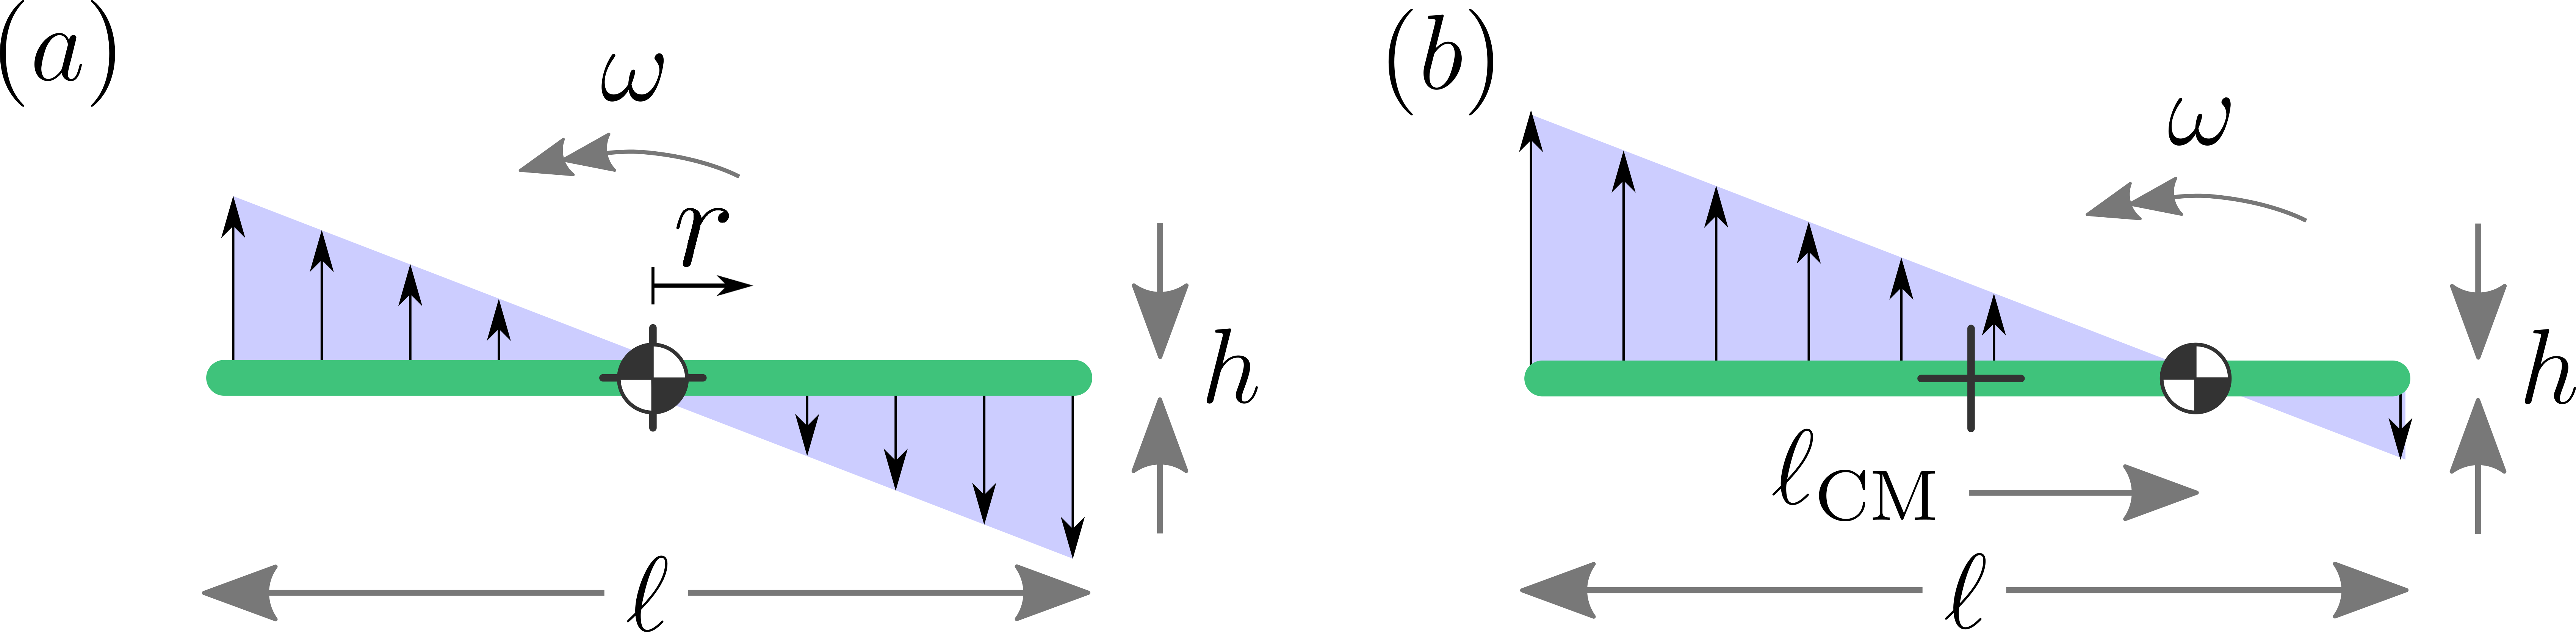
\includegraphics[width=0.8\textwidth]{pics/T_R_diagram1_2.png}
    \caption{Calculation of $\tau_\textnormal{R}$ with none or chordwise CoM displacement, according to \ref{eq:t_r_andersen} (a) and \ref{eq:t_r_li} (b). As the plate experiences pure rotation velocity about the CoM ($\omega$), the drag force is integrated chordwise (shown in blue) for $-\frac{\ell}{2} \le r \le \frac{\ell}{2}$. The force at each point $dr$ along the length of $r$ depends on the point velocity $v_n$; for (a) $v_n = \omega r$ and for (b) $v_n = \omega(r + \ell_{\textup{CM}})$.}
    \label{fig:t_r_diagram_1}
\end{figure*}

Introducing chordnormal CoM displacement makes this integration more complex, since the angle of motion of each segment relative to the fluid is no longer constant across the plate:

\begin{figure*}
    \centering
    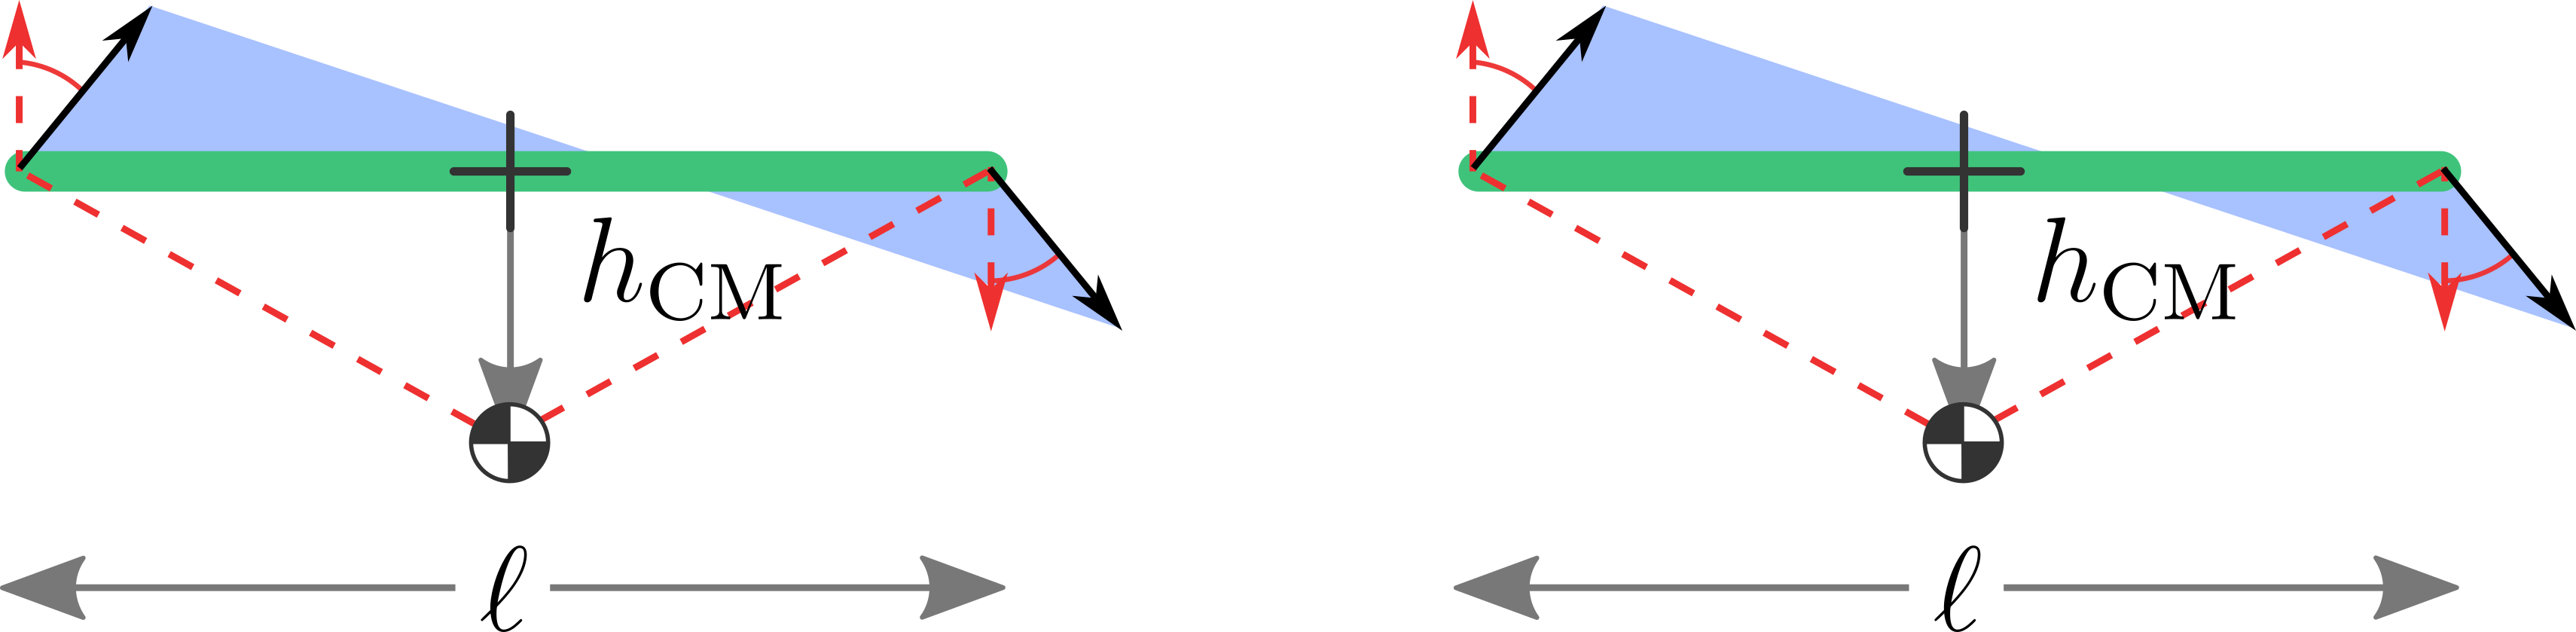
\includegraphics[width=0.7\textwidth]{pics/g12.png}
    \caption{Calculation of $\tau_\textnormal{R}$ with chordnormal CoM displacement.}
    \label{fig:t_r_diagram_2}
\end{figure*}

To derive the new integral, I will start from the definition of the derivative (local torque-induced drag) of \ref{eq:t_r_andersen} from (\cite{andersen2005analysis}, p19):

\begin{equation}
d \tau_\textnormal{R} = -\frac{1}{2}\rho_f C_{\textup{D}}^{\pi /2} v_n  \left| v_n \right| r\hspace{1mm}dr\label{eq:t_r_andersen_2}
\end{equation}

Where $v_n$ is the velocity of each segment, and $r$ is the position along the plate relative to the center. By integrating over $\ell$ we obtain the expression for $\tau_\textnormal{R}$:

\begin{equation}
\tau_\textnormal{R} = - \frac{1}{2}\rho_f C_{\textup{D}}^{\pi /2} \int_{\ell/2}^{-\ell/2}  v_n  \left| v_n \right| r dr\label{eq:simplified_tr_integral}
\end{equation} 

Substituting $v_n = \omega r$ simplifies down to \ref{eq:t_r_andersen} as required:

\begin{equation}
\tau_\textnormal{R} = -\frac{1}{2}\rho_f C_{\textup{D}}^{\pi /2} \int_{\ell/2}^{-\ell/2} \omega  \left| \omega \right| r^2 \left| r \right|  dr = -\frac{1}{64}\rho_f C_{\textup{D}}^{\pi /2}  \omega  \left| \omega \right|  \ell^4 
\end{equation}

For chordnormal CoM displacement, $v_n = \omega\sqrt{r^2+h_{\textup{CM}}^2}\cos(\tan^{-1}(\frac{h_{\textup{CM}}}{r}))$ which was found to be equivalent to $v_n = \omega r$. In other words, the chordnormal displacement of the CoM (by only considering the broadside-on velocity components) has no effect on the aerodynamic resistance to rotation. We can therefore use the chordwise definition \ref{eq:t_r_li} without incorporating the chordnormal displacement.

\section{Results}
The model equations have been implemented in a matlab script which can be found \href{https://github.com/ckessler2/phd/blob/main/Chornormal_Li_Model/Run_Li_Model.m}{here}. The aerodynamic coefficients have been optimised for \textit{Alsomitra} diaspores, and the initial conditions are $[0; 0; 0; pi/3; 0; 0]$ ($x,y,\theta,v_{x'},v_{y'},\omega$). The results comparing the Li model ($e_x = 0$) to the chordnormal model ($e_x=0$, $e_y = 0.2$) are shown on the next page.


\begin{figure}
    \centering
    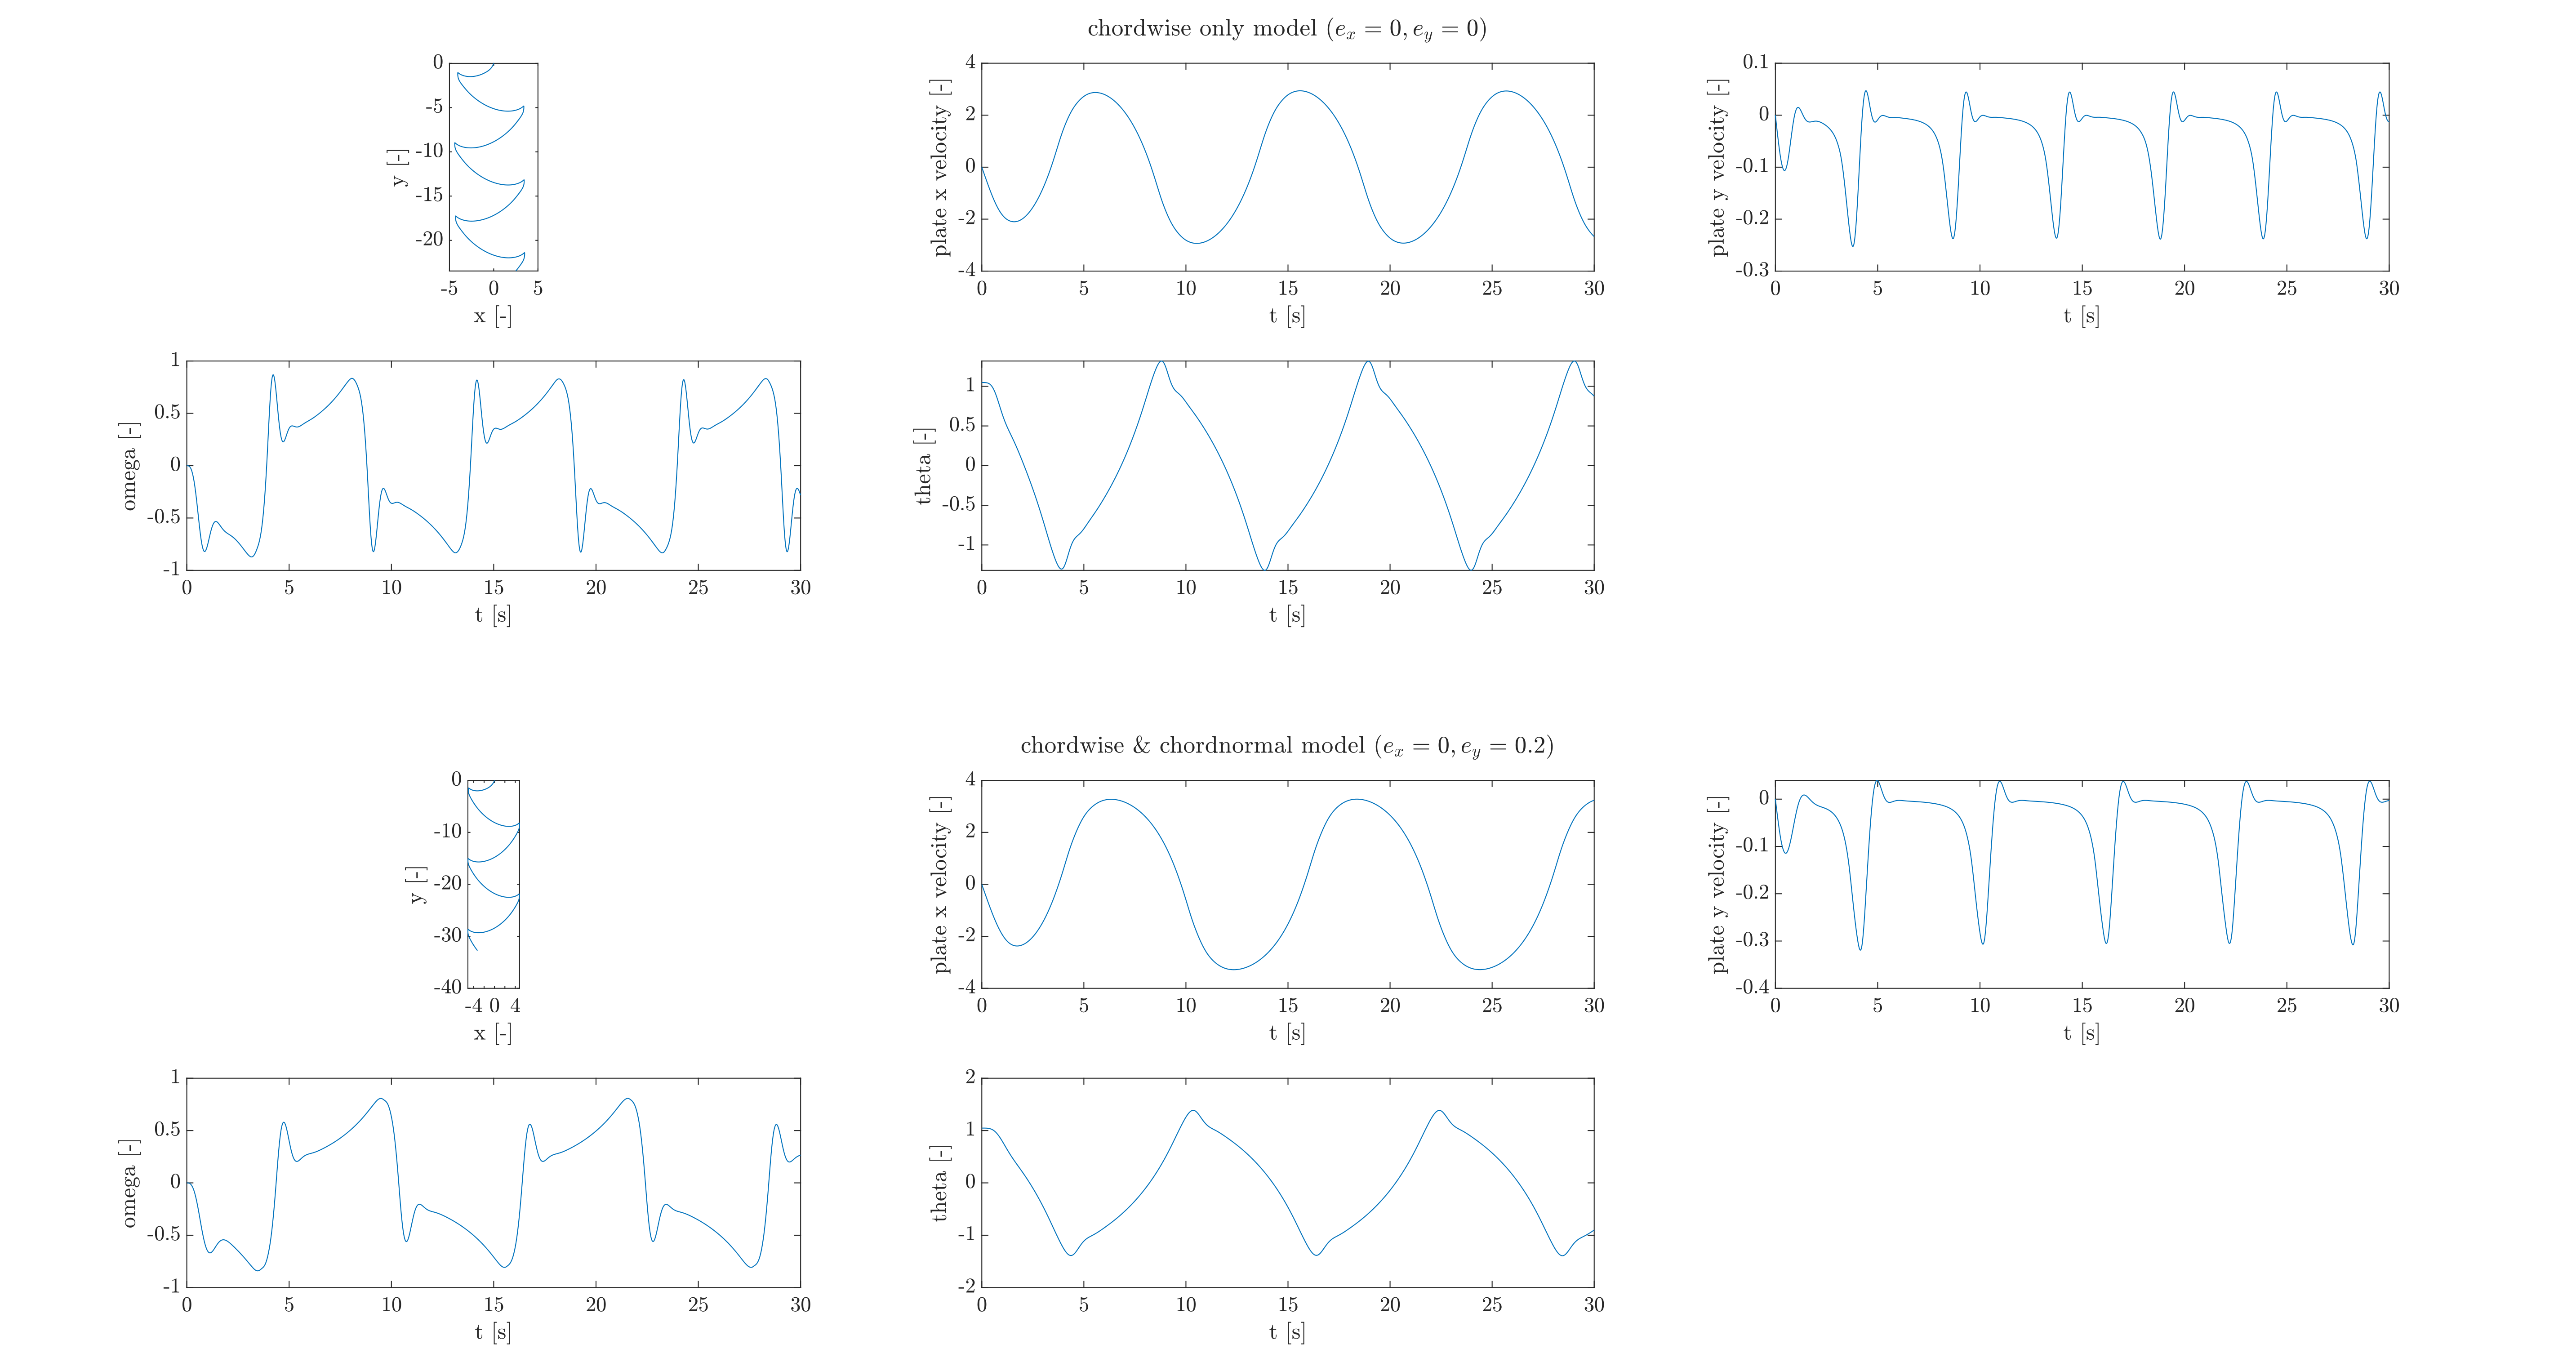
\includegraphics[angle=90,width=0.8\textwidth]{pics/g338.png}
    \label{fig:t_r_diagram_1}
\end{figure}

\textbf{}

% A similar derivative can be defined for chordwise CoM displacement, assuming $2e_x  \leq  1$ (CoM lies within the plate). From figure \ref{fig:t_r_diagram_1} we can see that the force distribution is translated up based on the velocity of the CoM ($\omega\ell_{\textup{CM}} $). Substituting $v_n = \omega(r + \ell_{\textup{CM}})$ and $r = r + \ell_{\textup{CM}}$ (??) into \ref{eq:simplified_tr_integral}:

% \begin{equation}
% \tau_\textnormal{R} = -\frac{1}{2}\rho_f C_{\textup{D}}^{\pi /2} \omega  \left| \omega \right| \int_{\ell/2}^{-\ell/2}( r + \ell_{\textup{CM}})^2 \left| r + \ell_{\textup{CM}} \right| dr 
% \end{equation}

% % \begin{equation}
% % = \frac{1}{2}\rho_f C_{\textup{D}}^{\pi /2}  \omega  \left| \omega \right| \left (\int_{\ell/2}^{-\ell/2}\ell^3 d\ell
% % + \int_{\ell/2}^{-\ell/2} 3\ell_{\textup{CM}}^2\ell d\ell 
% % + \int_{\ell/2}^{-\ell/2} 3\ell_{\textup{CM}}\ell^2 d\ell 
% % +  \int_{\ell/2}^{-\ell/2} \ell_{\textup{CM}}^3 d\ell  \right)
% % \end{equation}

% \begin{equation}
% = -\frac{1}{2}\rho_f C_{\textup{D}}^{\pi /2}  \omega  \left| \omega \right| \left[\left( 
% \frac{(\ell_{\textup{CM}}+\frac{l}{2})^4}{4}
% \right)+\left( 
% \frac{(\ell_{\textup{CM}}-\frac{l}{2})^4}{4}
% \right)\right]
% \end{equation}

% \begin{align*}
%     = &-\frac{1}{2}\rho_f  C_{\textup{D}}^{\pi /2}  \omega  \left| \omega \right|  \left(
%      \left [ 
%     \frac{\ell_{\textup{CM}}^4}{4}+\frac{ \ell_{\textup{CM}}^3\ell}{2}+\frac{3\ell_{\textup{CM}}^2\ell^2+\ell_{\textup{CM}}\ell^3}{8}+\frac{\ell^4}{64}
%     \right] \right.\\
%     & +
%     \left. \left [ 
%     \frac{\ell_{\textup{CM}}^4}{4}-\frac{ \ell_{\textup{CM}}^3\ell}{2}+\frac{3\ell_{\textup{CM}}^2\ell^2-\ell_{\textup{CM}}\ell^3}{8}+\frac{\ell^4}{64}
%     \right]
%     \right)
% \end{align*}

% \begin{equation}
% = -\frac{1}{2}\rho_f  C_{\textup{D}}^{\pi /2}  \omega  \left| \omega \right| \left (
% \frac{\ell_{\textup{CM}}^4}{2}
% +\frac{3\ell_{\textup{CM}}^2\ell^2}{4}
% +\frac{\ell^4}{32}
% \right )
% \end{equation}



% \begin{equation}
% = -\frac{1}{128}\rho_f  \ell^4  C_{\textup{D}}^{\pi /2}  \omega  \left| \omega \right| \left (
% 2  + \frac{48\ell_{\textup{CM}}^2}{\ell^2} + \frac{32\ell_{\textup{CM}}^4}{\ell^4 }
% \right )
% \end{equation}


% \begin{equation}
% = -\frac{1}{128}\rho_f\ell^4 C_{\textup{D}}^{\pi /2} \omega  \left| \omega \right| \left [ \left ( \frac{2\ell_{\textup{CM}}}{\ell}+1 \right )^4 +\left ( \frac{2\ell_{\textup{CM}}}{\ell}-1 \right )^4\right ]
% \end{equation}

\bibliographystyle{jfm}
% Note the spaces between the initials
\bibliography{References}

\end{document}
Alsomitra - CORA overview (Copy)